%; whizzy paragraph -pdf xpdf -latex ./whizzypdfptex.sh
%; whizzy-paragraph "^\\\\begin{frame}"
% latex beamer presentation.
% platex, latex-beamer でコンパイルすることを想定。 

%     Tokyo Debian Meeting resources
%     Copyright (C) 2009 Junichi Uekawa
%     Copyright (C) 2009 Nobuhiro Iwamatsu

%     This program is free software; you can redistribute it and/or modify
%     it under the terms of the GNU General Public License as published by
%     the Free Software Foundation; either version 2 of the License, or
%     (at your option) any later version.

%     This program is distributed in the hope that it will be useful,
%     but WITHOUT ANY WARRANTY; without even the implied warranty of
%     MERCHANTABILITY or FITNESS FOR A PARTICULAR PURPOSE.  See the
%     GNU General Public License for more details.

%     You should have received a copy of the GNU General Public License
%     along with this program; if not, write to the Free Software
%     Foundation, Inc., 51 Franklin St, Fifth Floor, Boston, MA  02110-1301 USA

\documentclass[cjk,dvipdfmx,12pt]{beamer}
\usetheme{Tokyo}
\usepackage{monthlypresentation}

%  preview (shell-command (concat "evince " (replace-regexp-in-string "tex$" "pdf"(buffer-file-name)) "&"))
%  presentation (shell-command (concat "xpdf -fullscreen " (replace-regexp-in-string "tex$" "pdf"(buffer-file-name)) "&"))
%  presentation (shell-command (concat "evince " (replace-regexp-in-string "tex$" "pdf"(buffer-file-name)) "&"))

%http://www.naney.org/diki/dk/hyperref.html
%日本語EUC系環境の時
\AtBeginDvi{\special{pdf:tounicode EUC-UCS2}}
%シフトJIS系環境の時
%\AtBeginDvi{\special{pdf:tounicode 90ms-RKSJ-UCS2}}

\title{Debian での数学ことはじめ。}
\subtitle{gnuplot, Octave, R 入門}
\author{まえだこうへい mkouhei@debian.or.jp \\IRC nick: mkouhei}
\date{2009年11月14日}
\logo{
\includegraphics[width=8cm]{image200607/openlogo-light.eps}}

%begin of commandline0
\newenvironment{commandline0}%
{\VerbatimEnvironment
  \begin{Sbox}\begin{minipage}{0.9\hsize}\begin{fontsize}{5}{5} \begin{BVerbatim}}%
{\end{BVerbatim}\end{fontsize}\end{minipage}\end{Sbox}
  \setlength{\fboxsep}{10pt}

\vspace{10pt}% skip before
\fcolorbox{dancerdarkblue}{dancerlightblue}{\TheSbox}

\vspace{6pt}% skip after
}
%end of commandline0

\begin{document}

\frame{\titlepage{}}

\begin{frame}{スプレッドシートって落ちません?}
\begin{itemize}
 \item データ量増えてくるとレスポンス最悪。
 \item 循環参照するとOOoなんて落ちる。
 \item OSまで固まるなんて最悪。
\end{itemize}

その他の不満。
\begin{itemize}
 \item 組み込み関数の精度がそもそも怪しい。
 \item テキストデータじゃないから、diff できないし。\\
       \texttt{git diff --binary}できるけど、読めん!
\end{itemize}
\end{frame}

\begin{frame}{魂の叫びが聞こえそうです。}
 \begin{minipage}[t]{0.45\hsize}
  \huge{もうこんな生活嫌だ!}
 \end{minipage}
 \begin{minipage}[t]{0.45\hsize}
  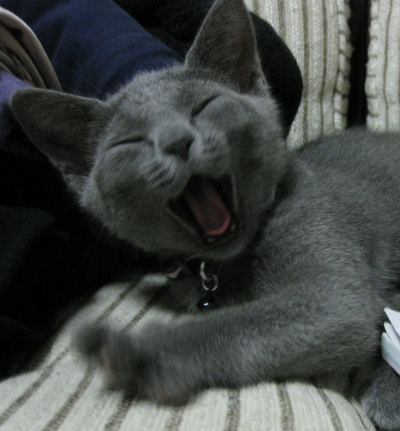
\includegraphics[width=1\hsize]{image200911/komame.png}
 \end{minipage}
\end{frame}

\begin{frame}{今日の献立。}
\begin{itemize}
\item gnuplot
\item GNU Octave
\item GNU R
\end{itemize}

以上、三本をお送りします。
\end{frame}

\begin{frame}{特徴。}
\begin{itemize}
 \item gnuplot
      \begin{itemize}
       \item グラフ描画が得意なコ。
       \item 外部プログラムから呼び出せます。
       \item LaTeXとも連携できちゃいます。
      \end{itemize}
 \item GNU Octave
       \begin{itemize}
	\item 数値計算が得意なコ。
	\item グラフ描画は gnuplot 使います。
	\item MATLAB の互換を目指してます。\footnote{別の見方ではMATLAB
	      のクローン(clone)なんだとか。}
       \end{itemize}
 \item GNU R
       \begin{itemize}
	\item 統計処理が得意なコ。
	\item 拡張機能が豊富です。
	\item グラフ描画機能もあります。
       \end{itemize}
\end{itemize}
\end{frame}

\begin{frame}[containsverbatim]{インストール方法。}
gnuplot

\begin{commandline}
$ sudo apt-get install gnuplot
\end{commandline}

GNU Octave

\begin{commandline}
$ sudo apt-get install octave3.2
\end{commandline}

GNU R

\begin{commandline}
$ sudo apt-get install r-base
\end{commandline}

\end{frame}

\begin{frame}[containsverbatim]{今月の具材。}
我が家の光熱費
\begin{commandline}
"date","days","kWh","kWh/d","yen/d","yen","days","m^3","m^3/d","yen/d","yen","days","m^3","m^3/d","yen/d","yen","yen/d","yen"
2001/04,11,34,3.09,83.5,918,36,4.9,0.14,108.3,3900,58,9,0.16,22.8,1320,,
2001/05,33,95,2.88,73.8,2434,29,3.5,0.12,114.1,3310,,,,,,,
2001/06,30,129,4.3,102.7,3082,32,3,0.09,96.9,3100,61,3,0.05,15.7,960,,
2001/07,28,155,5.54,131.3,3676,28,1.7,0.06,91.1,2550,,,,,,,
(snip)
\end{commandline}

 image200911/konetsu.csv にあるので、手元に勉強会のリポジトリがある人は試
 してみると良いよ。
\end{frame}

\begin{frame}{今月の具材。}
我が家の光熱費
\begin{itemize}
 \item 2001年4月から2009年9月までのデータ。
 \item 2回大きく変わる。大雑把に把握しているのは、以下。
 \item 2006年9月に市川から多摩に引越し。
       \begin{itemize}
	\item 電気契約が30Aから40Aに。
	\item ガスがプロパンから都市ガスに。
	\item 水道代が上がる&下水道代が追加に。
       \end{itemize}
 \item 2008年10月に結婚。
       \begin{itemize}
	\item ガス、水道使用量が倍増。
	\item 電気使用量はあまり変わらず。
       \end{itemize}
\end{itemize}
\end{frame}


\begin{frame}[containsverbatim]{gnuplotで処理した場合。}
基本は、データのプロット。\\
setで行っているのはグラフの見栄えが主。

 \begin{minipage}{0.45\hsize}
 \begin{commandline0}
reset
set terminal epslatex input color
set output "gnuplot.tex"
set datafile separator ","
set xdata time
set timefmt "%Y/%m"
set format x "%Y/%m"
set xtics rotate by -90
set mxtics 12
set xrange ["2001/04":"2009/08"]
set yrange [0:400]
set xlabel "年月"
set ylabel "電気使用量 [kWh]"
set y2range [0:50]
set y2label "ガス・水道使用量 [立方メートル]"
set ytics nomirror
set y2tics
plot "kohnetsuhi.csv" using 1:3 axes x1y1 \
  title "電気" with line,\
  "" using 1:8 axes x1y2 title "ガス" with line,\
  "" using 1:13 axes x1y2 title "水道" with line
 \end{commandline0}
 \end{minipage}
 \begin{minipage}{0.45\hsize}
  \scalebox{0.5}[0.5]{% GNUPLOT: LaTeX picture with Postscript
\begingroup
  \makeatletter
  \providecommand\color[2][]{%
    \GenericError{(gnuplot) \space\space\space\@spaces}{%
      Package color not loaded in conjunction with
      terminal option `colourtext'%
    }{See the gnuplot documentation for explanation.%
    }{Either use 'blacktext' in gnuplot or load the package
      color.sty in LaTeX.}%
    \renewcommand\color[2][]{}%
  }%
  \providecommand\includegraphics[2][]{%
    \GenericError{(gnuplot) \space\space\space\@spaces}{%
      Package graphicx or graphics not loaded%
    }{See the gnuplot documentation for explanation.%
    }{The gnuplot epslatex terminal needs graphicx.sty or graphics.sty.}%
    \renewcommand\includegraphics[2][]{}%
  }%
  \providecommand\rotatebox[2]{#2}%
  \@ifundefined{ifGPcolor}{%
    \newif\ifGPcolor
    \GPcolortrue
  }{}%
  \@ifundefined{ifGPblacktext}{%
    \newif\ifGPblacktext
    \GPblacktexttrue
  }{}%
  % define a \g@addto@macro without @ in the name:
  \let\gplgaddtomacro\g@addto@macro
  % define empty templates for all commands taking text:
  \gdef\gplbacktext{}%
  \gdef\gplfronttext{}%
  \makeatother
  \ifGPblacktext
    % no textcolor at all
    \def\colorrgb#1{}%
    \def\colorgray#1{}%
  \else
    % gray or color?
    \ifGPcolor
      \def\colorrgb#1{\color[rgb]{#1}}%
      \def\colorgray#1{\color[gray]{#1}}%
      \expandafter\def\csname LTw\endcsname{\color{white}}%
      \expandafter\def\csname LTb\endcsname{\color{black}}%
      \expandafter\def\csname LTa\endcsname{\color{black}}%
      \expandafter\def\csname LT0\endcsname{\color[rgb]{1,0,0}}%
      \expandafter\def\csname LT1\endcsname{\color[rgb]{0,1,0}}%
      \expandafter\def\csname LT2\endcsname{\color[rgb]{0,0,1}}%
      \expandafter\def\csname LT3\endcsname{\color[rgb]{1,0,1}}%
      \expandafter\def\csname LT4\endcsname{\color[rgb]{0,1,1}}%
      \expandafter\def\csname LT5\endcsname{\color[rgb]{1,1,0}}%
      \expandafter\def\csname LT6\endcsname{\color[rgb]{0,0,0}}%
      \expandafter\def\csname LT7\endcsname{\color[rgb]{1,0.3,0}}%
      \expandafter\def\csname LT8\endcsname{\color[rgb]{0.5,0.5,0.5}}%
    \else
      % gray
      \def\colorrgb#1{\color{black}}%
      \def\colorgray#1{\color[gray]{#1}}%
      \expandafter\def\csname LTw\endcsname{\color{white}}%
      \expandafter\def\csname LTb\endcsname{\color{black}}%
      \expandafter\def\csname LTa\endcsname{\color{black}}%
      \expandafter\def\csname LT0\endcsname{\color{black}}%
      \expandafter\def\csname LT1\endcsname{\color{black}}%
      \expandafter\def\csname LT2\endcsname{\color{black}}%
      \expandafter\def\csname LT3\endcsname{\color{black}}%
      \expandafter\def\csname LT4\endcsname{\color{black}}%
      \expandafter\def\csname LT5\endcsname{\color{black}}%
      \expandafter\def\csname LT6\endcsname{\color{black}}%
      \expandafter\def\csname LT7\endcsname{\color{black}}%
      \expandafter\def\csname LT8\endcsname{\color{black}}%
    \fi
  \fi
  \setlength{\unitlength}{0.0500bp}%
  \begin{picture}(7200.00,5040.00)%
    \gplgaddtomacro\gplbacktext{%
      \csname LTb\endcsname%
      \put(1210,1408){\makebox(0,0)[r]{\strut{} 0}}%
      \put(1210,1829){\makebox(0,0)[r]{\strut{} 50}}%
      \put(1210,2250){\makebox(0,0)[r]{\strut{} 100}}%
      \put(1210,2671){\makebox(0,0)[r]{\strut{} 150}}%
      \put(1210,3092){\makebox(0,0)[r]{\strut{} 200}}%
      \put(1210,3513){\makebox(0,0)[r]{\strut{} 250}}%
      \put(1210,3934){\makebox(0,0)[r]{\strut{} 300}}%
      \put(1210,4355){\makebox(0,0)[r]{\strut{} 350}}%
      \put(1210,4776){\makebox(0,0)[r]{\strut{} 400}}%
      \put(1763,1276){\rotatebox{-90}{\makebox(0,0)[l]{\strut{}2002/01}}}%
      \put(2320,1276){\rotatebox{-90}{\makebox(0,0)[l]{\strut{}2003/01}}}%
      \put(2877,1276){\rotatebox{-90}{\makebox(0,0)[l]{\strut{}2004/01}}}%
      \put(3436,1276){\rotatebox{-90}{\makebox(0,0)[l]{\strut{}2005/01}}}%
      \put(3994,1276){\rotatebox{-90}{\makebox(0,0)[l]{\strut{}2006/01}}}%
      \put(4551,1276){\rotatebox{-90}{\makebox(0,0)[l]{\strut{}2007/01}}}%
      \put(5107,1276){\rotatebox{-90}{\makebox(0,0)[l]{\strut{}2008/01}}}%
      \put(5667,1276){\rotatebox{-90}{\makebox(0,0)[l]{\strut{}2009/01}}}%
      \put(6122,1408){\makebox(0,0)[l]{\strut{} 0}}%
      \put(6122,2082){\makebox(0,0)[l]{\strut{} 10}}%
      \put(6122,2755){\makebox(0,0)[l]{\strut{} 20}}%
      \put(6122,3429){\makebox(0,0)[l]{\strut{} 30}}%
      \put(6122,4102){\makebox(0,0)[l]{\strut{} 40}}%
      \put(6122,4776){\makebox(0,0)[l]{\strut{} 50}}%
      \put(440,3092){\rotatebox{90}{\makebox(0,0){\strut{}$BEE5$;HMQNL(B [kWh]}}}%
      \put(6759,3092){\rotatebox{90}{\makebox(0,0){\strut{}$B%,%9!&?eF;;HMQNL(B [$BN)J}%a!<%H%k(B]}}}%
      \put(3666,154){\makebox(0,0){\strut{}$BG/7n(B}}%
    }%
    \gplgaddtomacro\gplfronttext{%
      \csname LTb\endcsname%
      \put(5003,4603){\makebox(0,0)[r]{\strut{}$BEE5$(B}}%
      \csname LTb\endcsname%
      \put(5003,4383){\makebox(0,0)[r]{\strut{}$B%,%9(B}}%
      \csname LTb\endcsname%
      \put(5003,4163){\makebox(0,0)[r]{\strut{}$B?eF;(B}}%
    }%
    \gplbacktext
    \put(0,0){\includegraphics{image200911/gnuplot.eps}}%
    \gplfronttext
  \end{picture}%
\endgroup
}
 \end{minipage}
\end{frame}

\begin{frame}[containsverbatim]{gnuplotで処理した場合。}
基本は、データのプロット。\\
setで行っているのはグラフの見栄えが主。

 \begin{commandline0}
reset                                        # 設定の初期化
set terminal epslatex input color            # EPS LaTeX でカラー出力
set output "gnuplot.tex"                     # ファイル名 gnuplot.tex で保存
set datafile separator ","                   # 読み込むデータファイルはカンマ区切り
set xdata time                               # x軸のパラメータは時間データ
set timefmt "%Y/%m"                          # 読み込む時間データの書式
set format x "%Y/%m"                         # 出力するx軸の書式を指定
set xtics rotate by -90                      # x軸のメモリラベルを-90度回転
set mxtics 12                                # x軸の補助メモリの間隔
set xrange ["2001/04":"2009/08"]             # x軸のデータ範囲
set yrange [0:400]                           # y軸のデータ範囲
set xlabel "年月"                            # x 軸のラベル
set ylabel "電気使用量 [kWh]"                 # y軸の名前
set y2range [0:50]                           # 第2y軸のデータ範囲
set y2label "ガス・水道使用量 [立方メートル]"  # 第2y軸のラベル
set ytics nomirror                           # 第2y軸は右側のみに表示
set y2tics                                   # 第2y軸を表示
plot "kohnetsuhi.csv" using 1:3 axes x1y1 \  # 第1,3列のデータでx軸、y軸で表示
  title "電気" with line,\                    # 凡例のタイトルと線プロット
  "" using 1:8 axes x1y2 title "ガス" with line,\ 
  "" using 1:13 axes x1y2 title "水道" with line
 \end{commandline0}
\end{frame}

\begin{frame}[containsverbatim]{gnuplotでの処理。}
gnuplot を起動してバッチをロード。

\begin{commandline}
$ gnuplot
> load ``gnuplot.gp''
> exit
$ ls
gnuplot.eps gnuplot.tex
\end{commandline}

これを LaTeXで取り込むと、先ほどのような図に。
\begin{itemize}
 \item デフォルトでは、別ウィンドウで表示される。
 \item 3次元グラフならグルグル回転もできる。
 \item 他の画像フォーマットにも出力できる。
\end{itemize}
\end{frame}

\begin{frame}[containsverbatim]{GNU Rでの処理。}
データの取り込み。
\begin{commandline}
$ R
> konetsu <- read.csv("konetsu.csv")
\end{commandline}

データのプロット。
\begin{commandline}
> plot(konetsu$kWh, type="l", ylim=c(0,400), ann=F)
> par(new=T)
> plot(konetsu$m.3, type="l", ylim=c(0,400), ann=F, col="red")
> par(new=T)
> plot(konetsu$m.3.1, ylim=c(0,400), ann=F, col="blue")
\end{commandline}
\end{frame}

\begin{frame}{GNU Rでの処理。}
 \begin{minipage}{0.45\hsize}
\begin{figure}[H]
 \includegraphics[width=0.9\hsize]{image200911/gnur.eps}
\end{figure}
\end{minipage}
 \begin{minipage}{0.45\hsize}
gnuplot のときに比べ、
\begin{itemize}
 \item 第2y軸を表示していない。
 \item ラベル表示していない。
\item 水道使用量が線じゃない。
\end{itemize}
といったのは、GNU Rのせいではありません。\\
私のカルマが足りないだけです。
\end{minipage}

\end{frame}

\begin{frame}[containsverbatim]{GNU Rでの処理。}
電気とガスの使用量の相関関係を見てみる。
\begin{commandline}

> cor.test(konetsu$kWh, konetsu$m.3)

	Pearson's product-moment correlation

data:  konetsu$kWh and konetsu$m.3 
t = 1.3154, df = 100, p-value = 0.1914
alternative hypothesis: true correlation is not equal to 0 
95 percent confidence interval:
 -0.06572595  0.31685457 
sample estimates:
      cor 
0.1304159 
\end{commandline}
 まあ、分かっていたことですがかなり低いです。平均気温となら、いずれかは相
 関関係があるかもしれません。
\end{frame}

\begin{frame}{GNU Octave での処理。}

{\huge 力及ばず。}

\end{frame}

\emtext{Debian パッケージ化に関して。}
\begin{frame}{拡張パッケージあります。}
 \begin{itemize}
  \item GNU Octave は、Octave-Forge。
  \item GNU Rは、CRAN(the Conprehensive R Archive Network)
  \item Perl のCPANのようなもん。
 \end{itemize}
\end{frame}

\begin{frame}[containsverbatim]{拡張パッケージを deb パッケージにする。}
既に結構debパッケージになっているけど全てじゃない。
\begin{commandline}
$ apt-cache search "GNU R" | wc -l
213
$ apt-cache search octave | wc -l
133
\end{commandline}

\end{frame}

\begin{frame}{拡張パッケージを deb パッケージにする。}
 deb パッケージにするためのパッケージが用意されている。
 \begin{itemize}
  \item Octave は、octave-pkg-dev。
	\begin{itemize}
	 \item debian/control の Build-Depends に octave-pkg-dev, \\
	       Depends に \$\{octave\:Depends\}を追記。
	 \item debian/rues に ``include
	       /usr/share/cdbs/1/class/octave-pkg.mk''を追記。
	 \item Octave-Forge由来でない場合は、rulesに ``SOURCEFORGE=NO''
	       を追記。
	\end{itemize}
  \item R は、 r-base-dev。
	\begin{itemize}
	 \item Debian パッケージポリシーを考慮して、バイナリ形式の実行ファ
	       イルは、/usr/lib/R/bin/R.binaryに分離する必要がある。
	 \item とあったのだけど、よく分からず。Javaのようにバイナリコー
	       ドで配布されている、ということだろうか?
	 \item 教えて、エロいヒト。
	\end{itemize}
\end{itemize}
\end{frame}

\begin{frame}{まとめ}
\begin{itemize}
 \item gnuplot, GNU R, GNU Octave の導入方法。
 \item gnuplot, GNU R の簡単な使い方。
 \item 拡張パッケージの Debian パッケージ化の際の考慮。
 \item 統計処理については、月の平均気温との相関関係を出すつもりだった。
 \item が、気象庁のデータから引っ張ってくるのは結構面倒なので、今後やってみる。
\end{itemize}

\end{frame}


\end{document}

;;; Local Variables: ***
;;; outline-regexp: "\\([ 	]*\\\\\\(documentstyle\\|documentclass\\|emtext\\|section\\|begin{frame}\\)\\*?[ 	]*[[{]\\|[]+\\)" ***
;;; End: ***
